\documentclass{scrreprt}
\usepackage{style}

\subject{Prüfung}
\title{107.A04 Wahrscheinlichkeitstheorie und stochastische Prozesse für Informatik 4.0}
\author{Byte Unit}
\uppertitleback{Unter GNU Free Document Lizenz}
\lowertitleback{\textcopyleft 2014 Byte Unit}
\date{04.03.2014}
%\publishers{}

\makeatletter
\AtBeginDocument{
    \hypersetup{
        pdftitle = {\@title},
        pdfsubject={\@subtitle},
        pdfauthor={\@author},
        pdfproducer={Latex (Debian/GNU Linux)},
        pdfkeywords={\@title, \@subject}
    }
}
\makeatother

%do some kind of magic :-)
\renewcommand{\thechapter}{\arabic{ExercPage}.}
\renewcommand{\newExercPage}{\exercPage
            \newpage
            \chapter{Übung}}
\ExerciseLevelInToc{section}

\renewcommand{\reference}[3]{#1 (siehe #2 im Skriptum)}

\setcounter{tocdepth}{5}

\begin{document}

\begin{uebsp}
\begin{Exercise}[label=ex:1.1]
Ein Würfel wird dreimal geworfen. $X$ sei das Minimum der drei Augenzahlen, $Y$ das Maximum. Bestimmen Sie die gemeinsame Verteilung von $X$ und $Y$, die Randverteilungen und Erwartungswerte.
\end{Exercise}
\begin{Answer}
    \begin{enumerate}[1.]
        \item Schritt: 4 Fälle betrachten:
                \begin{enumerate}[I)]
                    \item $X=z=Y\;\Rightarrow\;$1 Permutation ($\dfrac{3!}{3!}$)\\
                        z.B. kann $1=1=1$ nur durch eine Würfelknstellation/Permuation entstehen: $(1,1,1)$
                    \item $X=z<Y\;\Rightarrow\;$3 Permutationen ($\dfrac{3!}{2!}$)\\
                        z.B. kann $1=1<2$ nur durch 3 Würfelknstellationen/Permuationen entstehen: $(1,1,2),(1,2,1),(2,1,1)$
                    \item $X<z=Y\;\Rightarrow\;$3 Permutationen ($\dfrac{3!}{2!}$)\\
                        z.B. kann $1<2=2$ nur durch 3 Würfelknstellationen/Permuationen entstehen: $(1,2,2),(2,2,1),(2,1,2)$
                    \item $X<z<Y\;\Rightarrow\;$6 Permutationen ($\dfrac{3!}{1!}$)\\
                        z.B. kann $2<3<4$ durch folgende 6 Würfelkonstellationen/Permutationen entstehen:
                        $(2,3,4)$, $(2,4,3)$, $(3,2,4)$, $(3,4,2)$, $(4,2,3)$, $(4,3,2)$
                \end{enumerate}
        \item Wahrscheinlichkeitstabelle erstellen:
            Achtung, die Werte in der folgenden Tabelle müssen noch mit $\frac{1}{216}$ multipliziert werden!
            \begin{center}
            \begin{tabular}{|c||c|c|c|c|c|c||c|}
                \hline
                \diagbox{$y=$}{$x=$} & $1$ & $2$ & $3$ & $4$ & $5$ & $6$ & $\sum$\\ 
                \hline
                \hline
                $1$ & \cellcolor{orange!15}\fcolorbox{green}{orange!15}{\color{blue}$1$} &\cellcolor{orange!15} {\color{blue}$0$} &\cellcolor{orange!15} $0$ & $0$ & $0$ & $0$ & $1$\\
                \hline
                $2$ & \cellcolor{orange!15}\fcolorbox{green}{orange!15}{\color{blue}$6$} & \cellcolor{orange!15}{\color{blue}$1$} & \cellcolor{orange!15}$0$ & $0$ & $0$ & $0$ & $7$\\
                \hline
                $3$ & \fcolorbox{green}{white}{\color{blue}$12$} & {\color{blue}$6$} & $1$ & $0$ & $0$ & $0$ & $19$\\
                \hline
                $4$ & \fcolorbox{green}{white}{$18$} & $12$ & $6$ & $1$ & $0$ & $0$ & $37$\\
                \hline
                $5$ & $24$ & $18$ & $12$ & $6$ & $1$ & $0$ & $61$\\
                \hline
                $6$ & $30$ & $24$ & $18$ & $12$ & $6$ & $1$ & $91$\\
                \hline
                \hline
                $\sum$ & $91$ & $61$ & $37$ & $19$ & $7$ & $1$ & $216$\\
                \hline
            \end{tabular}
            \end{center}
            Diese Tabelle zeigt für jede $x/y$-Kombination die Wahrscheinlichkeit an.
            z.B: $x=4$ und $y=5$ hat die Wahrscheinlichkeit $\frac{6}{216}$.

            Man sieht hier auch gut, dass die Wahrscheinlichkeit, dass $x>y$ ist immer 0 ist.

            Die rechteste Spalte und die unterste Zeile sind die Randwahrscheinlichkeiten.

        \item Verteilungstabelle erstellen:
            Dazu werden die Werte der vorderen Tabelle verwendet:

            \begin{center}
            \begin{tabular}{|c|c|c|c|c|c|c|c|c|}
                \hline
                $\mathbb P_{X,Y}(x,y)$ & $x<2$ & $x<3$ & $x<4$ & $x<5$ & $x<6$ & $x< \infty$\\ 
                \hline
                $y<2$ &     $1$  & $1$   & $1$   & $1$   & $1$   & $1$\\
                \hline
                $y<3$ &     $7$  & $8$   & \cellcolor{orange!15}$8$   & $8$   & $8$   & $8$\\
                \hline
                $y<4$ &     $19$ & {\color{blue}$26$}  & $27$  & $27$  & $27$  & $27$\\
                \hline
                $y<5$ &     \fcolorbox{green}{white}{$37$} & $56$  & $63$  & $64$  & $64$  & $64$\\
                \hline
                $y<6$ &     $61$ & $98$  & $117$ & $124$ & $125$ & $125$\\
                \hline
                $y<\infty$& $91$ & $152$ & $189$ & $208$ & $215$ & $216$\\
                \hline
            \end{tabular}
            \end{center}

            Der blaue Wert entsteht beispielsweise durch die Summierung aller Blauen Zahlen in der vorigen Tabelle. Der grün eingerahmte durch die Summation der grün eingerahmten Werte und der orange hinterlegte Wert durch die Summe der Orange hinterlegten Werte. usw.

            \textbf{Die Zeile mit $y<\infty$ bzw. die Spalte mit $x<\infty$ sind die Randverteilungen.}

            \begin{center}
            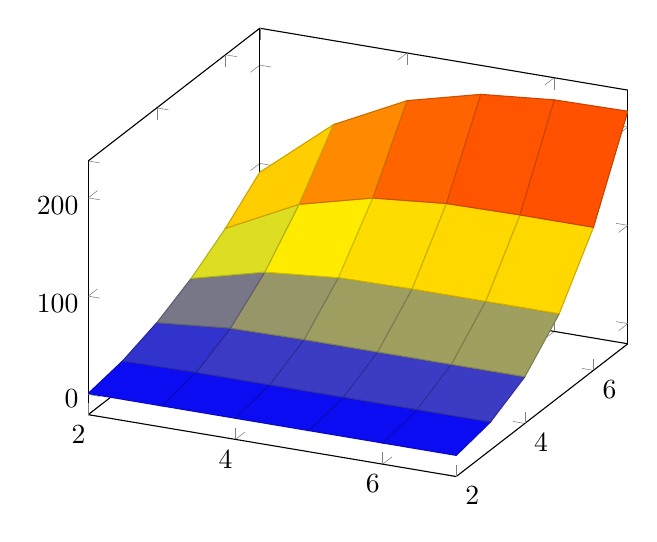
\begin{tikzpicture} 
            \begin{axis} 
            \addplot3[surf] coordinates{
                    (2,2,1)  (2,3,7)  (2,4,19)  (2,5,37)  (2,6,61)   (2,7,91)
                                                                                
                    (3,2,1)  (3,3,8)  (3,4,26)  (3,5,56)  (3,6,98)   (3,7,152)
                                                                                
                    (4,2,1)  (4,3,8)  (4,4,27)  (4,5,63)  (4,6,117)  (4,7,189)
                                                                                
                    (5,2,1)  (5,3,8)  (5,4,27)  (5,5,64)  (5,6,124)  (5,7,208)

                    (6,2,1)  (6,3,8)  (6,4,27)  (6,5,64)  (6,6,125)  (6,7,215)

                    (7,2,1)  (7,3,8)  (7,4,27)  (7,5,64)  (7,6,125)  (7,7,216)
            };
            \end{axis}
            \end{tikzpicture}
            \end{center}

            \begin{center}
                \begin{tikzpicture}[scale=0.85]
                    {
    \begin{axis}[domain=0:8,
            axis x line=bottom, % no box around the plot, only x and y axis
            axis y line=left, % the * would suppress the arrow tips
            xlabel=Augenzahl,
            %ylabel=Wahrscheinlichkeit,
            legend pos=north west,
            samples=50,
            height=6cm,
            width=10cm,
            clip=false]
            \addplot[blue] coordinates{(-1,0)(1,0)};
            \addlegendentry[align=left]{Randverteilung $x$};
            \addplot[blue,forget plot] coordinates{(1, 91)(2, 91)};
            \addplot[blue,forget plot] coordinates{(2,152)(3,152)};
            \addplot[blue,forget plot] coordinates{(3,189)(4,189)};
            \addplot[blue,forget plot] coordinates{(4,208)(5,208)};
            \addplot[blue,forget plot] coordinates{(5,215)(6,215)};
            \addplot[blue,forget plot] coordinates{(6,216)(8,216)};

            \draw[dotted] (axis cs:1,  0) -- (axis cs:1,  91);
            \draw[dotted] (axis cs:2, 91) -- (axis cs:2,152);
            \draw[dotted] (axis cs:3,152) -- (axis cs:3,189);
            \draw[dotted] (axis cs:4,189) -- (axis cs:4,208);
            \draw[dotted] (axis cs:5,208) -- (axis cs:5,215);
            \draw[dotted] (axis cs:6,215) -- (axis cs:6,216);
            \addplot[discontinuityblue,forget plot] coordinates{(1,0)(2,91)(3,152)(4,189)(5,208)(6,215)};
            \addplot[continuityblue,forget plot] coordinates{(1,91)(2,152)(3,189)(4,208)(5,215)(6,216)};


            \addplot[red] coordinates{(-1,0)(1,0)};
            \addlegendentry[align=left]{Randwahrscheinlichkeit $x$};%TODO: add better label
            \addplot[red,forget plot] coordinates{(1,91)(2,91)};
            \addplot[red,forget plot] coordinates{(2,61)(3,61)};
            \addplot[red,forget plot] coordinates{(3,37)(4,37)};
            \addplot[red,forget plot] coordinates{(4,19)(5,19)};
            \addplot[red,forget plot] coordinates{(5, 7)(6, 7)};
            \addplot[red,forget plot] coordinates{(6, 1)(7, 1)};
            \addplot[red,forget plot] coordinates{(7, 0)(8, 0)};

            \draw[dotted] (axis cs:1,  0) -- (axis cs:1,  91);
            \draw[dotted] (axis cs:2,  91) -- (axis cs:2,  61);
            \draw[dotted] (axis cs:3,  61) -- (axis cs:3, 37);
            \draw[dotted] (axis cs:4, 37) -- (axis cs:4, 19);
            \draw[dotted] (axis cs:5, 19) -- (axis cs:5,7);
            \draw[dotted] (axis cs:6, 7) -- (axis cs:6,1);            
            \draw[dotted] (axis cs:7, 1) -- (axis cs:7,0);            
            \addplot[discontinuityred,forget plot] coordinates{(1,0)(2,91)(3,61)(4,37)(5,19)(6,7)(7,1)};
            \addplot[continuityred,forget plot] coordinates{(1,91)(2,61)(3,37)(4,19)(5,7)(6,1)(7,0)};
    \end{axis}
}

                \end{tikzpicture}
            \end{center}

            \begin{center}
                \begin{tikzpicture}[scale=0.85]
                    {
    \begin{axis}[domain=0:8,
            axis x line=bottom, % no box around the plot, only x and y axis
            axis y line=left, % the * would suppress the arrow tips
            xlabel=Augenzahl,
            %ylabel=Wahrscheinlichkeit,
            legend pos=north west,
            samples=50,
            height=6cm,
            width=10cm,
            clip=false]
            \addplot[blue] coordinates{(-1,0)(1,0)};
            \addlegendentry[align=left]{Randverteilung $y$};
            \addplot[blue,forget plot] coordinates{(1,  1)(2,  1)};
            \addplot[blue,forget plot] coordinates{(2,  8)(3,  8)};
            \addplot[blue,forget plot] coordinates{(3, 27)(4, 27)};
            \addplot[blue,forget plot] coordinates{(4, 64)(5, 64)};
            \addplot[blue,forget plot] coordinates{(5,125)(6,125)};
            \addplot[blue,forget plot] coordinates{(6,216)(8,216)};

            \draw[dotted] (axis cs:1,  0) -- (axis cs:1,  1);
            \draw[dotted] (axis cs:2,  1) -- (axis cs:2,  8);
            \draw[dotted] (axis cs:3,  8) -- (axis cs:3, 27);
            \draw[dotted] (axis cs:4, 27) -- (axis cs:4, 64);
            \draw[dotted] (axis cs:5, 64) -- (axis cs:5,125);
            \draw[dotted] (axis cs:6,125) -- (axis cs:6,216);
            \addplot[discontinuityblue,forget plot] coordinates{(1,0)(2,1)(3,8)(4,27)(5,64)(6,125)};
            \addplot[continuityblue,forget plot] coordinates{(1,1)(2,8)(3,27)(4,64)(5,125)(6,216)};


            \addplot[red] coordinates{(-1,0)(1,0)};
            \addlegendentry[align=left]{Randwahrscheinlichkeit $y$};%TODO: add better label
            \addplot[red,forget plot] coordinates{(1,  1)(2,  1)};
            \addplot[red,forget plot] coordinates{(2,  7)(3,  7)};
            \addplot[red,forget plot] coordinates{(3, 19)(4, 19)};
            \addplot[red,forget plot] coordinates{(4, 37)(5, 37)};
            \addplot[red,forget plot] coordinates{(5, 61)(6, 61)};
            \addplot[red,forget plot] coordinates{(6, 91)(7, 91)};
            \addplot[red,forget plot] coordinates{(7, 0)(8, 0)};

            \draw[dotted] (axis cs:1,  0) -- (axis cs:1,  1);
            \draw[dotted] (axis cs:2,  1) -- (axis cs:2,  7);
            \draw[dotted] (axis cs:3,  7) -- (axis cs:3, 19);
            \draw[dotted] (axis cs:4, 19) -- (axis cs:4, 37);
            \draw[dotted] (axis cs:5, 37) -- (axis cs:5,61);
            \draw[dotted] (axis cs:6, 61) -- (axis cs:6,91);            
            \draw[dotted] (axis cs:7, 0) -- (axis cs:7,91);            
            \addplot[discontinuityred,forget plot] coordinates{(1,0)(2,1)(3,7)(4,19)(5,37)(6,61)(7,91)};
            \addplot[continuityred,forget plot] coordinates{(1,1)(2,7)(3,19)(4,37)(5,61)(6,91)(7,0)};
    \end{axis}
}

                \end{tikzpicture}
            \end{center}

        \item Erwartungswert für $x$:
            \[\frac{1\cdot 91+2\cdot 61+3\cdot 37+4\cdot 19+5\cdot 7+6\cdot 1}{216}\approx2.042\]
        \item Erwartungswert für $y$:
            \[\frac{1\cdot 1+2\cdot 7+3\cdot 19+4\cdot 37+5\cdot 61+6\cdot 91}{216}\approx4.958\]

        \item Schritt: Bestimmen der Wahrscheinlichkeit für X=k (nicht wirklich notwendig, nur der Vollständigkeit halber):
            \[X=1:\;1\cdot I+5\cdot II+5\cdot III+10\cdot IV=1\cdot1+5\cdot3+5\cdot3+10\cdot6=91\]
                \[\Rightarrow\mathbb{P}(X=1)=\frac{91}{216}\approx \;\;42.13\%\]
            \[X=2:\;1\cdot I+4\cdot II+4\cdot III+6\cdot IV=1\cdot1+4\cdot3+4\cdot3+6\cdot6=61\]
                \[\Rightarrow\mathbb{P}(X=2)=\frac{61}{216}\approx 28.24\%\]
            \[X=3:\;1\cdot I+3\cdot II+3\cdot III+3\cdot IV=1\cdot1+3\cdot3+3\cdot3+3\cdot6=37\]
                \[\Rightarrow\mathbb{P}(X=3)=\frac{37}{216}\approx 17.13\%\]
            \[X=4:\;1\cdot I+2\cdot II+2\cdot III+1\cdot IV=1\cdot1+2\cdot3+2\cdot3+1\cdot6=19\]
                \[\Rightarrow\mathbb{P}(X=4)=\frac{19}{216}\approx 8.80\%\]
            \[X=5:\;1\cdot I+1\cdot II+1\cdot III+0\cdot IV=1\cdot1+1\cdot3+1\cdot3+0\cdot6=7\]
                \[\Rightarrow\mathbb{P}(X=5)=\frac{7}{216}\approx 3.24\%\]
            \[X=6:\;1\cdot I+0\cdot II+0\cdot III+0\cdot IV=1\cdot1+0\cdot3+0\cdot3+0\cdot6=1\]
                \[\Rightarrow\mathbb{P}(X=6)=\frac{1}{216}\approx \;\;0.46\%\]
        \item Verteilungsfunktion $F_X(x)$ (nicht wirklich notwendig, nur der Vollständigkeit halber):
            \begin{multicols}{2}

                \begin{tikzpicture}[scale=0.85]
                    {
    \begin{axis}[domain=0:8,
            axis x line=bottom, % no box around the plot, only x and y axis
            axis y line=left, % the * would suppress the arrow tips
            xlabel=Augenzahl,
            ylabel=Prozent,
            legend pos=north west,
            samples=50,
            height=6cm,
            width=10cm,
            clip=false]
            \addplot[blue] coordinates{(-1,0)(1,0)};
            \addlegendentry[align=left]{Vert.fkt. $f_X(x)$};%TODO: add a better label
            \addplot[blue,forget plot] coordinates{(1,42.13)(2,42.13)};
            \addplot[blue,forget plot] coordinates{(2,70.37)(3,70.37)};
            \addplot[blue,forget plot] coordinates{(3,87.50)(4,87.50)};
            \addplot[blue,forget plot] coordinates{(4,96.30)(5,96.30)};
            \addplot[blue,forget plot] coordinates{(5,99.54)(6,99.54)};
            \addplot[blue,forget plot] coordinates{(6,100)(8,100)};

            \draw[dotted] (axis cs:1,0) -- (axis cs:1,42.13);
            \draw[dotted] (axis cs:2,42.13) -- (axis cs:2,70.37);
            \draw[dotted] (axis cs:3,70.37) -- (axis cs:3,87.50);
            \draw[dotted] (axis cs:4,87.50) -- (axis cs:4,96.30);
            \draw[dotted] (axis cs:5,96.30) -- (axis cs:5,99.54);
            \draw[dotted] (axis cs:6,99.54) -- (axis cs:6,100);
            \addplot[discontinuityblue,forget plot] coordinates{(1,0)(2,42.13)(3,70.37)(4,87.50)(5,96.30)(6,99.54)};
            \addplot[continuityblue,forget plot] coordinates{(1,42.13)(2,70.37)(3,87.50)(4,96.30)(5,99.54)(6,100)};


            \addplot[red] coordinates{(-1,0)(1,0)};
            \addlegendentry[align=left]{Vert. diskret};%TODO: add better label
            \addplot[red,forget plot] coordinates{(1,42.13)(2,42.13)};
            \addplot[red,forget plot] coordinates{(2,28.24)(3,28.24)};
            \addplot[red,forget plot] coordinates{(3,17.13)(4,17.13)};
            \addplot[red,forget plot] coordinates{(4,8.8)(5,8.8)};
            \addplot[red,forget plot] coordinates{(5,3.24)(6,3.24)};
            \addplot[red,forget plot] coordinates{(6,0.46)(7,0.46)};
            \addplot[red,forget plot] coordinates{(7,0)(8,0)};

            \draw[dotted] (axis cs:1,0) -- (axis cs:1,42.13);
            \draw[dotted] (axis cs:2,42.13) -- (axis cs:2,28.24);
            \draw[dotted] (axis cs:3,28.24) -- (axis cs:3,17.13);
            \draw[dotted] (axis cs:4,17.13) -- (axis cs:4,8.8);
            \draw[dotted] (axis cs:5,8.8) -- (axis cs:5,3.24);
            \draw[dotted] (axis cs:6,3.24) -- (axis cs:6,0.46);
            \draw[dotted] (axis cs:7,0.46) -- (axis cs:7,0);

            \addplot[discontinuityred,forget plot] coordinates{(1,0)(2,42.13)(3,28.24)(4,17.13)(5,8.8)(6,3.24)(7,0.46)};
            \addplot[continuityred,forget plot] coordinates{(1,42.13)(2,28.24)(3,17.13)(4,8.8)(5,3.24)(6,0.46)(7,0)};
    \end{axis}
}

                \end{tikzpicture}

                Die rote Linie gibt die Verteilung diskret an, während die blaue Linie die Verteilungsfunktion $f_X(x)$ rechts darstellt.
            \columnbreak
            \[f_X(x) = \begin{cases} 
                        0 &\mbox{wenn } x < 1 \\
                        \frac{91}{216}\approx 42.13\% & \mbox{wenn } x < 2\\
                        \frac{152}{216}\approx 70.37\% & \mbox{wenn } x < 3\\
                        \frac{189}{216}\approx 87.50\% & \mbox{wenn } x < 4\\
                        \frac{208}{216}\approx 96.30\% & \mbox{wenn } x < 5\\
                        \frac{215}{216}\approx 99.54\% & \mbox{wenn } x < 6\\
                        \frac{216}{216}\approx 100\% & \mbox{wenn } x < 7 
                        \end{cases}\]
            \end{multicols}
        \item Bestimmen der Wahrscheinlichkeit für $Y=k$ (nicht wirklich notwendig, nur der Vollständigkeit halber):
            Diese ist die selbe Verteilungsfunktion wie für $X=k$ nur in umgekehrter Reihenfolge:
            \[Y=1:\;1\cdot I+0\cdot II+0\cdot III+0\cdot IV=1\cdot1+0\cdot3+0\cdot3+0\cdot6=1\]
                \[\Rightarrow\mathbb{P}(X=6)=\frac{1}{216}\approx \;\;0.46\%\]
            \[Y=2:\;1\cdot I+1\cdot II+1\cdot III+0\cdot IV=1\cdot1+1\cdot3+1\cdot3+0\cdot6=7\]
                \[\Rightarrow\mathbb{P}(X=5)=\frac{7}{216}\approx 3.24\%\]
            \[Y=3:\;1\cdot I+2\cdot II+2\cdot III+1\cdot IV=1\cdot1+2\cdot3+2\cdot3+1\cdot6=19\]
                \[\Rightarrow\mathbb{P}(X=4)=\frac{19}{216}\approx 8.80\%\]
            \[Y=4:\;1\cdot I+3\cdot II+3\cdot III+3\cdot IV=1\cdot1+3\cdot3+3\cdot3+3\cdot6=37\]
                \[\Rightarrow\mathbb{P}(X=3)=\frac{37}{216}\approx 17.13\%\]
            \[Y=5:\;1\cdot I+4\cdot II+4\cdot III+6\cdot IV=1\cdot1+4\cdot3+4\cdot3+6\cdot6=61\]
                \[\Rightarrow\mathbb{P}(X=2)=\frac{61}{216}\approx 28.24\%\]
            \[Y=6:\;1\cdot I+5\cdot II+5\cdot III+10\cdot IV=1\cdot1+5\cdot3+5\cdot3+10\cdot6=91\]
                \[\Rightarrow\mathbb{P}(X=1)=\frac{91}{216}\approx \;\;42.13\%\]
        \item Verteilungsfunktion $F_Y(y)$ (nicht wirklich notwendig, nur der Vollständigkeit halber):
            \begin{multicols}{2}
                \begin{tikzpicture}[scale=0.85]
                    {
    \begin{axis}[domain=0:8,
            axis x line=bottom, % no box around the plot, only x and y axis
            axis y line=left, % the * would suppress the arrow tips
            xlabel=Augenzahl,
            ylabel=Prozent,
            legend pos=north west,
            samples=50,
            height=6cm,
            width=10cm,
            clip=false]
            \addplot[blue] coordinates{(-1,0)(1,0)};
            \addlegendentry[align=left]{Vert.fkt. $f_Y(y)$};%TODO: add a better label
            \addplot[blue,forget plot] coordinates{(1,0.46)(2,0.46)};
            \addplot[blue,forget plot] coordinates{(2,3.7)(3,3.7)};
            \addplot[blue,forget plot] coordinates{(3,12.5)(4,12.5)};
            \addplot[blue,forget plot] coordinates{(4,29.63)(5,29.63)};
            \addplot[blue,forget plot] coordinates{(5,57.87)(6,57.87)};
            \addplot[blue,forget plot] coordinates{(6,100)(8,100)};

            \draw[dotted] (axis cs:1,0) -- (axis cs:1,0.46);
            \draw[dotted] (axis cs:2,0.46) -- (axis cs:2,3.7);
            \draw[dotted] (axis cs:3,3.7) -- (axis cs:3,12.5);
            \draw[dotted] (axis cs:4,12.5) -- (axis cs:4,29.63);
            \draw[dotted] (axis cs:5,29.63) -- (axis cs:5,57.87);
            \draw[dotted] (axis cs:6,57.87) -- (axis cs:6,100);
            \addplot[discontinuityblue,forget plot] coordinates{(1,0)(2,0.46)(3,3.7)(4,12.5)(5,29.63)(6,57.87)};
            \addplot[continuityblue,forget plot] coordinates{(1,0.46)(2,3.7)(3,12.5)(4,29.63)(5,57.87)(6,100)};


            \addplot[red] coordinates{(-1,0)(1,0)};
            \addlegendentry[align=left]{Vert. diskret};%TODO: add better label
            \addplot[red,forget plot] coordinates{(1,0.46)(2,0.46)};
            \addplot[red,forget plot] coordinates{(2,3.24)(3,3.24)};
            \addplot[red,forget plot] coordinates{(3,8.8)(4,8.8)};
            \addplot[red,forget plot] coordinates{(4,17.13)(5,17.13)};
            \addplot[red,forget plot] coordinates{(5,28.24)(6,28.24)};
            \addplot[red,forget plot] coordinates{(6,42.24)(7,42.24)};
            \addplot[red,forget plot] coordinates{(7,0)(8,0)};

            \draw[dotted] (axis cs:1,0) -- (axis cs:1,0.46);
            \draw[dotted] (axis cs:2,0.46) -- (axis cs:2,3.24);
            \draw[dotted] (axis cs:3,3.24) -- (axis cs:3,8.8);
            \draw[dotted] (axis cs:4,8.8) -- (axis cs:4,17.13);
            \draw[dotted] (axis cs:5,17.13) -- (axis cs:5,28.24);
            \draw[dotted] (axis cs:6,28.24) -- (axis cs:6,42.24);
            \draw[dotted] (axis cs:7,42.24) -- (axis cs:7,0);

            \addplot[discontinuityred,forget plot] coordinates{(1,0)(2,0.46)(3,3.24)(4,8.8)(5,17.13)(6,28.24)(7,42.24)};
            \addplot[continuityred,forget plot] coordinates{(1,0.46)(2,3.24)(3,8.8)(4,17.13)(5,28.24)(6,42.24)(7,0)};
    \end{axis}
}

                \end{tikzpicture}

                Die rote Linie gibt die Verteilung diskret an, während die blaue Linie die Verteilungsfunktion $f_Y(y)$ rechts darstellt.
            \columnbreak
            \[f_Y(y) = \begin{cases} 
                        0 &\mbox{wenn } y < 1 \\
                        \frac{1}{216}\approx 0.46\% & \mbox{wenn } y < 2\\
                        \frac{8}{216}\approx 3.7\% & \mbox{wenn } y < 3\\
                        \frac{27}{216}\approx 12.5\% & \mbox{wenn } y < 4\\
                        \frac{64}{216}\approx 29.63\% & \mbox{wenn } y < 5\\
                        \frac{125}{216}\approx 57.87\% & \mbox{wenn } y < 6\\
                        \frac{216}{216}\approx 100\% & \mbox{wenn } y < 7 
                        \end{cases}\]
            \end{multicols}

    \end{enumerate}
\end{Answer}
\end{uebsp}

\begin{uebsp}
\begin{Exercise}[label=ex:1.2]
    Eine Markovkette mit vier Zuständen hat die Übergangsmatrix
    \[\left(\begin{array}{cccc}
        1 & 0 & 0 & 0\\
        0.2 & 0.4 & 0.2 & 0.2\\
        0.4 & 0.2 & 0.2 & 0.2\\
        0 & 0 & 0 & 1\\
    \end{array}\right)\]
    Bestimme Sie die Klassen von Zuständen, die Absorptionswahrscheinlichkeiten und die mittleren Absorptionszeiten.
\end{Exercise}
\begin{Answer}
\begin{enumerate}[i)]
    \item Klassen bilden:
        \begin{enumerate}[1)]
            \item Klasse $C_1$: $\{1\}$
            \item Klasse $C_2$: $\{4\}$
            \item Klasse $C_3$: $\{2,3\}$
        \end{enumerate}
    \item Bestimmen der Absorptionswahrscheinlichkeiten für Zustand $1$:
        \[a_i^{(1)}=\begin{cases}\sum_jp_{ij}a_j\\1&i=1\\0&i=\text{anderer absorbierender Zustand.}\end{cases}\]
        Somit können wir uns $a_2^{(1)}$, bzw. $a_3^{(1)}$ ausdrücken.
        \begin{eqnarray*}
            a_2^{(1)} &=& 0.2\cdot a_1^{(1)} + 0.4\cdot a_2^{(1)} + 0.2\cdot a_3^{(1)} + 0.2\cdot a_4^{(1)}\\
                &=&0.2\cdot 1 + 0.4\cdot a_2^{(1)} + 0.2\cdot a_3^{(1)} + 0.2\cdot 0=0.2 + 0.4\cdot a_2^{(1)} + 0.2\cdot a_3^{(1)}\\
            a_3^{(1)} &=& 0.4\cdot a_1^{(1)} + 0.2\cdot a_2^{(1)} + 0.2\cdot a_3^{(1)} + 0.2\cdot a_4^{(1)}=\\
                &=&0.4\cdot 1 + 0.2\cdot a_2^{(1)} + 0.2\cdot a_3^{(1)} + 0.2\cdot 0=0.4 + 0.2\cdot a_2^{(1)} + 0.2\cdot a_3^{(1)}
        \end{eqnarray*}

        Daraus erhalten wir 2 Gleichungen:
        \[0.4=-0.2a_2^{(1)}+0.8a_3^{(1)}\]
        \[0.2=0.6a_2^{(1)}-0.2a_3^{(1)}\]

        Diese werden mit Gauss gelöst:
        \[\left(\begin{array}{cc|c}
        -0.2 & 0.8 & 0.4\\
        0.6 & -0.2 & 0.2\\
        \end{array}\right)\xRightarrow{Z_2=Z_2+Z_1\cdot 3}
        \left(\begin{array}{cc|c}
        -0.2 & 0.8 & 0.4\\
        0 & 2.2 & 1.4\\
        \end{array}\right)\]
        $a_3^{(1)}$ berechnen:
        \[2.2\cdot a_3^{(1)}=1.4\;\Rightarrow\;a_3^{(1)}=\frac{1.4}{2.2}=\frac{7}{11}\]
        $a_2^{(1)}$ berechnen:
        \[-0.2\cdot a_2^{(1)}+0.8\cdot a_3^{(1)}=0.4\;\Rightarrow\;-0.2\cdot a_2^{(1)}+0.8\cdot \frac{7}{11}=0.4\;\Rightarrow\;\]
        \[-0.2\cdot a_2^{(1)}=\frac{44-56}{110}\;\Rightarrow\;a_2^{(1)}=\frac{12\cdot \cancel{10}}{11\cancel0\cdot 2}=\frac{6}{11}\]

    \item Bestimmen der Absorptionswahrscheinlichkeiten für Zustand $4$:
        Da es bei uns nur 2 absorbierende Zustände gibt, müssen die Absorptionswahrscheinlichkeiten in Summe 1 ergeben. Somit können wir uns die Absorptionswahrscheinlichkeiten berechnen, indem wir einfach die vorher berechneten Wahrscheinlichkeiten von 1 abziehen:

        Die Absorptionswahrscheinlichkeit $a_2^{(4)}$ lautet somit:
        \[a_2^{(4)}=1-a_2^{(1)}=\frac{11}{11}-\frac{6}{11}=\frac{5}{11}\]

        Die Absorptionswahrscheinlichkeit $a_3^{(4)}$ lautet somit:
        \[a_3^{(4)}=1-a_3^{(1)}=\frac{11}{11}-\frac{7}{11}=\frac{4}{11}\]

        Zur Kontrolle werden wir aber trozdem noch die Wahrscheinlichkeiten mit der herkömmlichen Methode berechnen:
        \[a_i^{(4)}=\begin{cases}\sum_jp_{ij}a_j\\1&i=4\\0&i=\text{anderer absorbierender Zustand.}\end{cases}\]
        Somit können wir uns $a_2^{(4)}$, bzw. $a_3^{(4)}$ ausdrücken.
        \begin{eqnarray*}
            a_2^{(4)} &=& 0.2\cdot a_1^{(4)} + 0.4\cdot a_2^{(4)} + 0.2\cdot a_3^{(4)} + 0.2\cdot a_4^{(4)}\\
                &=&0.2\cdot 0 + 0.4\cdot a_2^{(4)} + 0.2\cdot a_3^{(4)} + 0.2\cdot 0=0.2 + 0.4\cdot a_2^{(4)} + 0.2\cdot a_3^{(4)}\\
            a_3^{(4)} &=& 0.4\cdot a_1^{(4)} + 0.2\cdot a_2^{(4)} + 0.2\cdot a_3^{(4)} + 0.2\cdot a_4^{(4)}=\\
                &=&0.4\cdot 0 + 0.2\cdot a_2^{(4)} + 0.2\cdot a_3^{(4)} + 0.2\cdot 1=0.2\cdot a_2^{(4)} + 0.2\cdot a_3^{(4)} + 0.2
        \end{eqnarray*}

        Daraus erhalten wir 2 Gleichungen:
        \[0.2=-0.2a_2^{(4)}+0.8a_3^{(4)}\]
        \[0.2=0.6a_2^{(4)}-0.2a_3^{(4)}\]

        Diese werden mit Gauss gelöst:
        \[\left(\begin{array}{cc|c}
        -0.2 & 0.8 & 0.2\\
        0.6 & -0.2 & 0.2\\
        \end{array}\right)\xRightarrow{Z_2=Z_2+Z_1\cdot 3}
        \left(\begin{array}{cc|c}
        -0.2 & 0.8 & 0.2\\
        0 & 2.2 & 0.8\\
        \end{array}\right)\]
        $a_3^{(4)}$ berechnen:
        \[2.2\cdot a_3^{(4)}=0.8\;\Rightarrow\;a_3^{(4)}=\frac{0.8}{2.2}=\frac{4}{11}\]
        $a_2^{(4)}$ berechnen:
        \[-0.2a_2^{(4)}+0.8a_3^{(4)}=0.2\;\Rightarrow\;-0.2a_2^{(4)}+0.8\cdot\frac{4}{11}=0.2\;\Rightarrow\]
        \[-0.2a_2^{(4)}=\frac{22-32}{110}\;\Rightarrow\;a_2^{(4)}=\frac{10\cdot \cancel{10}}{11\cancel0\cdot 2}=\frac{5}{11}\]
    \item Mittlere Absorptionszeiten:
        \[m_i=1+\sum_{j}p_{ij}m_j, i\neq i_0\;\;\text{sowie}\;\;m_{i_0}=0\]
        Somit wissen wir bereits: $m_1=0$ bzw. $m_4=0$.
        \[m_2=1+0.2\cdot m_1+0.4\cdot m_2+0.2\cdot m_3+0.2\cdot m_4=1+0.4\cdot m_2+0.2\cdot m_3\]
        \[0.6\cdot m_2=1+0.2\cdot m_3\;\Rightarrow\;0.6\cdot m_2-0.2\cdot m_3=1\]
        \[m_3=1+0.4\cdot m_1+0.2\cdot m_2+0.2\cdot m_3+0.2\cdot m_4=1+0.2\cdot m_2+0.2\cdot m_3\]
        \[0.8\cdot m_3=1+0.2\cdot m_2\;\Rightarrow\;0.8\cdot m_3-0.2\cdot m_2=1\]

        Somit haben wir 2 Gleichungen mit 2 Unbekannten:
        \[\left(\begin{array}{cc|c}
        -0.2 & 0.8 & 1\\
        0.6 & -0.2 & 1\\
        \end{array}\right)\xRightarrow{Z_2=Z_2+Z_1\cdot 3}
        \left(\begin{array}{cc|c}
        -0.2 & 0.8 & 1\\
        0 & 2.2 & 4\\
        \end{array}\right)\]
        \[2.2\cdot m_3=4\;\Rightarrow\;m_3=\frac{4}{2.2}=\frac{20}{11}\]
        \[-0.2\cdot m_2+0.8\cdot m_3=1\;\Rightarrow\;-0.2\cdot m_2=1-\frac{8}{\cancel{10}}\cdot \frac{2\cancel{0}}{11}=\frac{11}{11}-\frac{16}{11}=-\frac{5}{11}\;\Rightarrow\]
        \[\;m_2=\frac{5}{11}\cdot \frac{10}{2}=\frac{25}{11}\]

\end{enumerate}
\end{Answer}
\end{uebsp}
\begin{uebsp}
\begin{Exercise}[label=ex:1.3]
\end{Exercise}
Bestimmen Sie für die Verteilung $P=(0.10,0.30,0.15,0.10,0.20,0.15)$ den Huffman-, Shannon- und Fano-Code, die mittlere Unbestimmtheit und die Entropie.
\begin{Answer}
\begin{enumerate}[i)]
\item Entropie bestimmen:
    Denn diese ist für alle Codes die gleiche.
    \[H(P)=\sum_{i=1}^6p_i\log_2\left(\frac{1}{p_i}\right)\]
    \[H(P)=2\cdot 0.10\cdot\log_2\left(\frac{1}{0.1}\right)+2\cdot 0.15\cdot\log_2\left(\frac{1}{0.15}\right)+0.2\cdot\log_2\left(\frac{1}{0.2}\right)+0.3\cdot\log_2\left(\frac{1}{0.3}\right)\]
    \[H(P)\approx2.47\]
\item Huffman-Code:
    \begin{enumerate}[1)]
        \item nach Wahrscheinlichkeit aufsteigend sortieren:\\
            $P=(0.10,0.10,0.15,0.15,0.20,0.30)$
        \item Fasse die kleinsten Knoten $\{0.10, 0.10\}$ zusammen:
            \begin{center}
                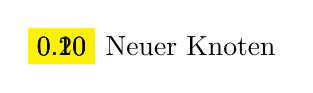
\begin{tikzpicture}[every tree node/.style={draw,circle},
                   level distance=1.25cm,sibling distance=.5cm, anchor=west,
                   edge from parent path={(\tikzparentnode) -- (\tikzchildnode)}]
                    \Tree [.\node[fill=yellow,label=east: {Neuer Knoten}] (A) {0.20} ; 
                    [.\node (B) {0.10}; ] [.\node (C) {0.10}; ] ]
                \end{tikzpicture}\\
            \end{center}

        \item Fasse die nächstkleineren Knoten $\{0.15, 0.15\}$ zusammen:
            \begin{center}
                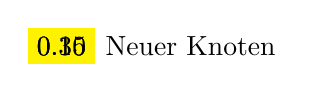
\begin{tikzpicture}[every tree node/.style={draw,circle},
                   level distance=1.25cm,sibling distance=.5cm, anchor=west,
                   edge from parent path={(\tikzparentnode) -- (\tikzchildnode)}]
                    \Tree [.\node[fill=yellow,label=east: {Neuer Knoten}] (A) {0.30} ; 
                    [.\node (B) {0.15}; ] [.\node (C) {0.15}; ] ]
                \end{tikzpicture}\\
            \end{center}

        \item Fasse die nächstkleineren Knoten $\{0.20(0.10+0.10), 0.20\}$ zusammen:
            \begin{center}
                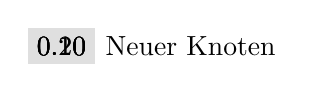
\begin{tikzpicture}[every tree node/.style={draw,circle},
                   level distance=1.25cm,sibling distance=.5cm, anchor=west,
                   edge from parent path={(\tikzparentnode) -- (\tikzchildnode)}]
                    \Tree [.\node[fill=yellow,label=east: {Neuer Knoten}] (A) {0.40} ; 
                    [.\node[fill=gray!25] (B) {0.20}; 
                        [.\node (B) {0.10}; ] [.\node (C) {0.10}; ] ] [.\node (C) {0.20}; ] ]
                \end{tikzpicture}\\
            \end{center}

        \item Fasse die nächstkleineren Knoten $\{0.30(0.15+0.15), 0.30\}$ zusammen:
            \begin{center}
                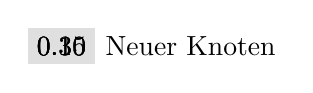
\begin{tikzpicture}[every tree node/.style={draw,circle},
                   level distance=1.25cm,sibling distance=.5cm, anchor=west,
                   edge from parent path={(\tikzparentnode) -- (\tikzchildnode)}]
                    \Tree [.\node[fill=yellow,label=east: {Neuer Knoten}] (A) {0.60} ; 
                    [.\node [fill=gray!25] (B) {0.30};
                        [.\node (B) {0.15}; ] [.\node (C) {0.15}; ] ] [.\node (C) {0.30};  ] ]
                \end{tikzpicture}\\
            \end{center}

        \item Fasse die verbleibenden Knoten $\{0.40, 0.60\}$ zusammen:
            \begin{center}
                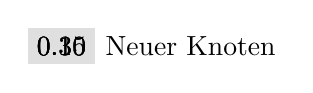
\begin{tikzpicture}[every tree node/.style={draw,circle},
                   level distance=1.25cm,sibling distance=.5cm, anchor=west,
                   edge from parent path={(\tikzparentnode) -- (\tikzchildnode)}]
                    \Tree [.\node[fill=yellow,label=east: {Neuer Knoten}] (A) {1.00} ; \edge node[auto=right] {\textcolor{blue}{1}}; 
                    [.\node[fill=gray!25] (A) {0.40} ;\edge node[auto=right] {\textcolor{blue}{1}}; 
                        [.\node[fill=gray!25] (B) {0.20};\edge node[auto=right] {\textcolor{blue}{1}}; 
                            [.\node (B) {0.10}; ]\edge node[auto=left] {\textcolor{blue}{0}}; [.\node (C) {0.10}; ] ]\edge node[auto=left] {\textcolor{blue}{0}}; [.\node (C) {0.20}; ] ]\edge node[auto=left] {\textcolor{blue}{0}}; [.\node[fill=gray!25] (A) {0.60} ;\edge node[auto=right] {\textcolor{blue}{1}}; 
                    [.\node [fill=gray!25] (B) {0.30};\edge node[auto=right] {\textcolor{blue}{1}};
                        [.\node (B) {0.15}; ]\edge node[auto=left] {\textcolor{blue}{0}}; [.\node (C) {0.15}; ] ]\edge node[auto=left] {\textcolor{blue}{0}}; [.\node (C) {0.30};  ]  ] ]
                \end{tikzpicture}\\
            \end{center}

        \item Codes bestimmen:
            \begin{center}
            \begin{tabular}{ccc}
                \hline
                Wahrscheinlichkeit $p_i$&Codewortlänge $l_i$ & Codewort $c_i$\\
                \hline
                $0.1$  & $3$ & $111$\\
                $0.1$  & $3$ & $110$\\
                $0.15$ & $3$ & $011$\\
                $0.15$ & $3$ & $010$\\
                $0.2$  & $2$ & $10$\\
                $0.3$  & $2$ & $00$\\
                \hline
            \end{tabular}
            \end{center}
        \item Mittlere Unbestimmtheit:
            \[H^*(P)=\sum_{i=1}^6p_il_i\]
            \[H^*(P)=0.3\cdot 2+0.2\cdot 2+2\cdot 0.15\cdot 3+2\cdot 0.1\cdot 3=2.5\]
    \end{enumerate}
    \item Shannon-Code
        \begin{enumerate}[1)]
            \item nach Wahrscheinlichkeit absteigend sortieren:\\
                $P=(0.30,0.20,0.15,0.15,0.10,0.10)$
            \item Verteilung $f_i$ und Codewortlänge $l_i$ berechnen: (mit den Formeln $f_i=\sum_j=1^i p_i$  bzw. $l_i=\lceil\log_2(1/p_i)\rceil$).
                \begin{center}
                    \begin{tabular}{ccc}
                        \hline
                        Wahrscheinlichkeit $p_i$&$l_i$ & $f_{i-1}$\\
                        \hline
                        $0.30$ & $2$ & $0$\\
                        $0.20$ & $3$ & $0.3$\\
                        $0.15$ & $3$ & $0.5$\\
                        $0.15$ & $3$ & $0.65$\\
                        $0.10$ & $4$ & $0.8$\\
                        $0.10$ & $4$ & $0.9$\\
                        \hline
                    \end{tabular}
                \end{center}
            \item Codewort $c_i$ bestimmen: (die $f_i$ in binär umgewandelt)
                 \begin{center}
                    \begin{tabular}{cccc}
                        \hline
                        Wahrscheinlichkeit $p_i$&$l_i$ & $f_{i-1}$ & $c_i$\\
                        \hline
                        $0.30$ & $2$ & $0$ & $00$\\
                        $0.20$ & $3$ & $0.3$ & $010$\\
                        $0.15$ & $3$ & $0.5$ & $100$\\
                        $0.15$ & $3$ & $0.65$ & $101$\\
                        $0.10$ & $4$ & $0.8$ & $1100$\\
                        $0.10$ & $4$ & $0.9$ & $1110$\\
                        \hline
                    \end{tabular}
                \end{center}                   
        \item Mittlere Unbestimmtheit:
            \[H^*(P)=\sum_{i=1}^6p_il_i\]
            \[H^*(P)=0.3\cdot 2+0.2\cdot 3+2\cdot 0.15\cdot 3+2\cdot 0.1\cdot 4=2.9\]
        \end{enumerate}
    \item Fanu-Code:
        \begin{enumerate}[1)]
            \item Gleich ohne sortieren die Codewortlängen $l_i$, die Verteilung $f_i$ sowie $\frac{f_{i-1}+f_i}{2}$ zu berechnen (wobei hier $l_i=\lceil\log_2(1/p_i)\rceil+1$)
                \begin{center}
                    \begin{tabular}{ccccc}
                        \hline
                        Wahrscheinlichkeit $p_i$&$l_i$ & $f_{i-1}$ & $f_{i}$\ & $\frac{f_i+f_{i-1}}{2}$\\
                        \hline
                        $0.10$ & $5$ & $0$ & $0.1$ & $0.05$\\
                        $0.30$ & $3$ & $0.1$ & $0.4$ & $0.25$\\
                        $0.15$ & $4$ & $0.4$ & $0.55$ & $0.475$\\
                        $0.10$ & $5$ & $0.55$ & $0.65$ & $0.6$\\
                        $0.20$ & $4$ & $0.65$ & $0.85$ & $0.75$\\
                        $0.15$ & $4$ & $0.85$ & $1.00$ & $0.925$\\
                        \hline
                    \end{tabular}
                \end{center}
            \item Codewort $c_i$ bestimmen: ($\frac{f_{i-1}+f_i}{2}$ in binär umgewandelt)
                 \begin{center}
                    \begin{tabular}{cccccc}
                        \hline
                        Wahrscheinlichkeit $p_i$&$l_i$ & $f_{i-1}$ & $f_{i}$\ & $\frac{f_i+f_{i-1}}{2}$ & $c_i$\\
                        \hline
                        $0.10$ & $5$ & $0$ & $0.1$ & $0.05$ & $00001$\\
                        $0.30$ & $3$ & $0.1$ & $0.4$ & $0.25$ & $010$\\
                        $0.15$ & $4$ & $0.4$ & $0.55$ & $0.475$ & $0111$\\
                        $0.10$ & $5$ & $0.55$ & $0.65$ & $0.6$ & $10011$\\
                        $0.20$ & $4$ & $0.65$ & $0.85$ & $0.75$ & $1100$\\
                        $0.15$ & $4$ & $0.85$ & $1.00$ & $0.925$ & $1110$\\
                        \hline
                    \end{tabular}
                \end{center}               
        \item Mittlere Unbestimmtheit:
            \[H^*(P)=\sum_{i=1}^6p_il_i\]
            \[H^*(P)=0.3\cdot 3+0.2\cdot 4+2\cdot 0.15\cdot 4+2\cdot 0.1\cdot 5=3.9\]
        \end{enumerate}
\end{enumerate}
\end{Answer}
\end{uebsp}

\begin{uebsp}
\begin{Exercise}[label=ex:1.4]
Ein Würfel wird 100-mal geworfen, mit den Häufigkeiten\\
\begin{center}
\begin{tabular}{|c|c|c|c|c|c|}
    \hline
    1 & 2 & 3 & 4 & 5 & 6\\
    \hline
    23 & 16 & 13 & 22 & 14 & 12\\
    \hline
\end{tabular}
\end{center}
Istder Würfel fair?
\end{Exercise}
\begin{Answer}
Wir sollen testen, ob es sich bei den Würfelergebnissen um eine Gleichverteilung handelt, mit $\mathbb P(X=1)=P(X=2)=...=P(X=6)=\frac{1}{6}$ und Erwartungswert $\mathbb E(X)=\frac{100}{6}=\frac{50}{3}$.

Die Häufigkeiten $y_k(y_1,...,y_6)$ geben an, wie oft $k$-Werte gewürfelt wurden.

Somit lautet unsere Nullhypothese $H_0$: die Häufigkeiten sind Gleichverteilt und der Würfel ist fair.
\begin{enumerate}[i)]
    \item Wir checken, ob die Faustregel erfüllt ist: $n\cdot p_i>5$
        \[n\cdot p_i=\frac{100}{6}=16.66...>5\]
    \item Ergebnis für 
        \[T=\sum_j=1^6\frac{(y_i-np_i)^2}{np_i}\]
        berechnen:
        \begin{center}
            \begin{tabular}{cccc}
                \hline
                $k$ & $y_i$ & $n\cdot p_i$ & $\frac{(y_i-np_i)^2}{np_i}$\\
                \hline
                $1$ & $23$ & $\frac{100}{6}=16.\overline 6$ & $\frac{(23-16.\overline{6})^2}{16.\overline{6}}=2.40\overline 6$ \\
                $2$ & $16$ & $\frac{100}{6}=16.\overline 6$ & $\frac{(16-16.\overline{6})^2}{16.\overline{6}}=0.02\overline 6$ \\
                $3$ & $13$ & $\frac{100}{6}=16.\overline 6$ & $\frac{(13-16.\overline{6})^2}{16.\overline{6}}=0.80\overline 6$ \\
                $4$ & $22$ & $\frac{100}{6}=16.\overline 6$ & $\frac{(22-16.\overline{6})^2}{16.\overline{6}}=1.70\overline 6$ \\
                $5$ & $14$ & $\frac{100}{6}=16.\overline 6$ & $\frac{(14-16.\overline{6})^2}{16.\overline{6}}=0.42\overline 6$ \\
                $6$ & $12$ & $\frac{100}{6}=16.\overline 6$ & $\frac{(12-16.\overline{6})^2}{16.\overline{6}}=1.30\overline 6$ \\
                \hline
                &&$\sum_{i=1}^6$&$2.40\overline 6 + 0.02\overline 6 + 0.80\overline 6 + 1.70\overline 6 + 0.42\overline 6 + 1.30\overline 6=6.68$
            \end{tabular}
        \end{center}
        Dieses Ergebnis muss nun mit $\chi^2_{5;0.95}$ verglichen werden:
        \[T=6.68<\chi^2_{5;0.95}=11.07\].

        Somit wird die Nullhypothese nicht verworfen.
\end{enumerate}
\end{Answer}
\end{uebsp}

\end{document}
